\chapter {Увоз Боричев}

Боричев увоз (или взвоз), он же, по различным летописным спискам – Зборичев, Биричев, Буричев, Оузборичев, Борищев, Оузборичев, Барнуев, Борнувье, Звозбори уев и так далее. Древняя дорога на Старокиевской горе, соединявшая нижний город Подол с верхним городом. Где был сей Боричев, и почему так назван?

Существует две основные версии его положения. Одна – давняя, поддерживаемая Берлинским, Максимовичем, Закревским, заключается в том, что увоз Боричев лежал в овраге, где теперь проходит фуникулер. По другой версии, любимой многими позднейшими историками, Боричев это нынешний Андреевский спуск.

Пора опровергнуть заблуждение относительно Андреевского, и дать обоснование тому, что Боричев это старинная дорога там, где нынче маршрут фуникулера, то бишь от Почтовой площади наверх к Михайловскому монастырю, воссозданному в конце 20 века, и зданию МИД. До сих пор, на 2021 год, сохранились упоминаемые в летописях и старинных грамотах урочища и местности.

Разберем по крупицам, с самого начала. В летописи как сказано? «И седяше Кый на горе, идеже ныне увоз Боричев».

Памятуя, что текст в летописях идет без пробелов между словами, а монахи переписывали всё, как могли распознать, предположу, что поначалу в подлиннике было нечто вроде (большими буквами выделено мною): «идеженынеУБОЗБоричев». То есть, «где ныне, убо (стало быть), Зборичев». Зборичев – от сборов, пошлин, ведь где-то внизу (изменение за века прибрежного русла не позволяют вычислить положение пристани в летописное время) находилась пристань, и купцы платили пошлину. Пошлина – слово емкое – платишь за прохождение.

Итак, есть вероятность, что слова «увоз» в первом варианте летописного рассказа не было. Просто на горе либо её склоне находилось место под названием Зборичев, где купцы, поднимаясь на гору платили сбор, пошлину. Более того, в дальнейшем летопись упоминает Боричев уже без «увоз» или «взвоз», а просто одним словом – Боричев, в разных его вариантах.

Но вернемся ко классическому толкованию, когда слово «увоз» всё же присутствует. К тому же всё равно нужна была дорога, путь соединения между верхом и низом.

Путаница первая. В старину словом «увоз» обозначали переправу либо перевоз. Реже, да и позже стали говорить в значении «спуск». Если около нынешней Почтовой площади была пристань, то и переправа. Это и вызвало давние, еще времен Нестора, сомнения в том, что Кий был не князем, но перевозчиком. Нестор опровергал: «не сведущие рекоша яко кий есть перевозник был. от киева бо бяше перевоз тогда с оной стороны днепра тем глаголаху на перевоз на киев».

Перевоз, переправа, увоз. Поэтому и увоз Боричев?

Между тем, в некоторых списках летописи вместо «увоз» стоит «взвоз». Взвоз – это подъем от чего-либо. Тоже вариант. Взвоз Боричев, Зборичев – дорога наверх, по ходу которой с купцов брали пошлину. Зборы, сборы, боры – от брать. Биричев – от того же, в одной грамоте сказано, «биривали» в значении «брали». Хотя известно и слово «бирич» – глашатай, объявлявший в народе княжеские приказы.

Но могла ли дорога в овраге между нынешней Почтовой площадью и верхом горы, то есть по ходу фуникулера, служить путем для перемещения грузов? Величина уклона там составляет 18-20 градусов. Возникает вопрос о том, как пользовались дорогой. Вот пристань, к ней прибывают корабли с грузами. Грузы с пристани доставлялись наверх вручную? Или купцы нанимали возы?

Летом 2013 года я катался в том краю на велике и хотел съехать по улице Боричев спуск, частично параллельной фуникулеру. Пришлось резко тормозить и спешиться, ибо живым я бы до конца улицы не добрался – слишком круто.

Тогда я задумался – если летописный увоз Боричев проходил по месту фуникулера, как оттуда съезжали и поднимались на возах? Продолжая рассуждать в таком духе, я поначалу пришел к мысли, что дорога наверх шла не прямо, а изгибами взбиралась по террасам холма. Рассуждения без знания местности могут завести к правдоподобной выдумке. Лишь подробное изучение окрестностей и сопоставление со старинными письменными свидетельствами дало мне четкое представление о Боричеве.

На крутизну нынешнего подъема по ходу фуникулера указывают и сторонники версии об Андреевском спуске. Мол, непригодно для сообщения. Пешком еще можно, а вот грузы, да на возах – невозможно. Но раньше Боричев имел другой угол наклона, более пологий.

Чтобы дальше всё излагать четко, опишу словами местность и покажу карту.

Нас интересует северо-восточный склон Старокиевской горы, уступами нисходящий к Подолу в сторону Днепра. На самом верху, у края холма, на Михайловской площади, расположены здание МИДа и Михайловский собор. Между ними пространство, и около кромки холма – верхняя станция фуникулера. Оттуда по прямой, в овраге, фуникулер спускается к своей нижней станции.

На пригорке, где расположился МИД, раньше стоял идол Перуна, откуда его потом свергли и построили на его месте церковь святого Василия, по христианскому имени князя Владимира.

Ниже МИДа и Михайловского монастыря лежит терраса с теперь прогулочной дорогой, идущей сначала по Владимирской горке (под монастырем) и дальше в сторону Андреевской церкви, огибая её с востока и севера, чтобы затем соединиться с Андреевским спуском. Дорога проходит под фуникулером, немного ниже верхней его платформы. Когда появились эти террасы – история умалчивает.

Еще ниже по склону – терраса с улицей Боричев Ток, названной так по имени местности. От Боричева Тока круто вниз, к улице Сагайдачного и Почтовой площади, перпендикулярно отходит короткая улица Боричев спуск.

До 1869 года отдельной улицы Боричев спуск не было. Она являлась частью продолженной наверху горы Трехсвятительской улицы, не соединяясь с нею. После 1869 сей отрезок получил самостоятельность и название «Боричева ввоза».

Теперь карта. Я сделал прорисовку по аэрофотоснимку 1943 года. С тех пор расположение улиц не изменилось.
\vspace*{\fill}
\begin{center}
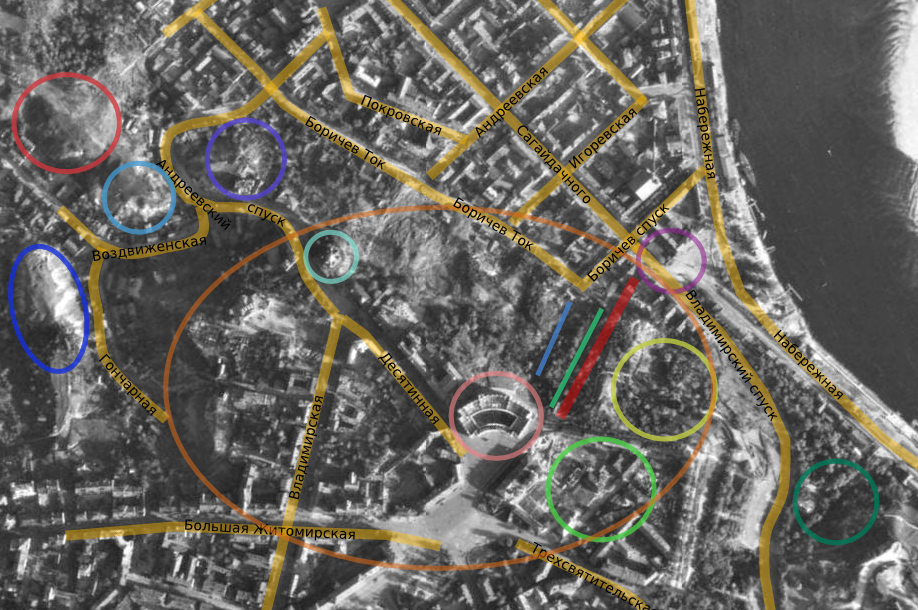
\includegraphics[width=\linewidth]{chast-colebanie-osnov/uvoz-borichev/bor-karta.jpg}
\end{center}
\vspace*{\fill}
\newpage

Линии:

\begin{itemize}
\item Красная – фуникулер, проложенный в частично засыпанном овраге. Это и есть увоз Боричев.

\item Зеленая рядом с ним – северо-западная сторона этого оврага, где видны остатки, и весьма явные, старинного вала. Вал сей продолжается почти до самого низа.

\item Голубая – чуть в отдалении от вала (снова на северо-запад) по склону сочился ручей, известный в прошлом как «Боричев поток» – отсюда и название нижележащей местности Боричев ток. Сейчас ручей перехвачен по склону дренажной системой, вода его весьма чиста, во всяком случае без запаха химии, а течение довольно бойкое.
\end{itemize}

Кружки:

\begin{itemize}
\item Розовый – здание МИД. Довлеет над окрестностями.

\item Бордовый – Почтовая площадь.

\item Желтый – Владимирская горка.

\item Салатовый – Михайловский монастырь.

\item Зеленый – Хрещатое (Крещатое) урочище, там где лестница к памятнику Магдебургскому праву.

\item Бирюзовый – Андреевская церковь.

\item Фиолетовый – гора Уздыхальница.

\item Голубой – гора Клинец.

\item Красный – гора Замковая.

\item Синий – гора Детинка.

\item Оранжевый – Киевица, Старокиевская.
\end{itemize}

Давайте подробно пройдемся по всей местности и обсудим её. Посмотрим, где и как она находит отражение в летописях, старинных грамотах, на давних картах и фотографиях. 

\newpage

Вот сам фуникулер. Снято как раз с той дороги, что по террасе идет от Владимирской горки (под Михайловским монастырем) и далее, огибая склон, в сторону Андреевской церкви. Отметим вал слева. 
\vspace*{\fill}
\begin{center}
\includegraphics[width=\linewidth]{chast-colebanie-osnov/uvoz-borichev/\myimgprefix IMG_20131013_145318.jpg}
\end{center}
\vspace*{\fill}
Если на него встать и посмотреть вдоль, можно заметить, что проложен он по ровной линии. От вала налево начинается ложбина, где стекал Боричев поток.

Противоположный берег оврага с фуникулером – намного выше, чем вал. Откос этого берега и следы постепенного оползания почвы дают основания полагать, что некогда овраг в тех пределах был шире. Местность справа считается нынче Владимирской горкой.

Внизу, у Почтовой площади, видна арка нижней станции фуникулера, до которой около 140 метров. А до верхней – всего тридцать. Непосредственно слева за кадром находится будка тяговой подстанции. Ее стены служат туалетом для киевлян и гостей столицы, равно как и все окрестности.

\newpage

Теперь пройдем несколько шагов в сторону и поглядим наверх:

\begin{center}
\includegraphics[width=\linewidth]{chast-colebanie-osnov/uvoz-borichev/\myimgprefix borichev-IMG_20131013_145300.jpg}
\end{center}

Вот так над дорогой (напомню, что мы стоим на террасе) проложен фуникулер. Впереди, на пригорке, видим его верхнюю станцию. За нею правее будет здание МИД, а слева на том же уровне – Михайловский монастырь.

И здесь вдумчивый читатель поразится крутизне склона и воскликнет – нет! Древнее путище явно не могло здесь проходить.

А сделаем поправку на время. Сейчас да, уж больно круто. Но что здесь было раньше? Вернее, чего не было?

Пригорка. И земли под нами не было, был более глубоко залегавший овраг с дорогой.

Представьте, что вместо изображенного перед нами на фотографии –  в склон дальше уходит, прорезая его, овраг. И он существовал в таком виде, по крайней мере, до 17 века.

Закревский приводит слова «старика Вигеля», который сетовал, что Боричев увоз засыпали. На Плане Ушакова 1695 года Боричева нет, зато видно, как по, условно говоря, верхней площадке фуникулера тянется буерак. Сейчас там ровное место. Вид со стороны Днепра, боярак посередке, слева – Михайловский монастырь, к нему тогда примыкал еще Свято-софиевский девичий:

\begin{center}
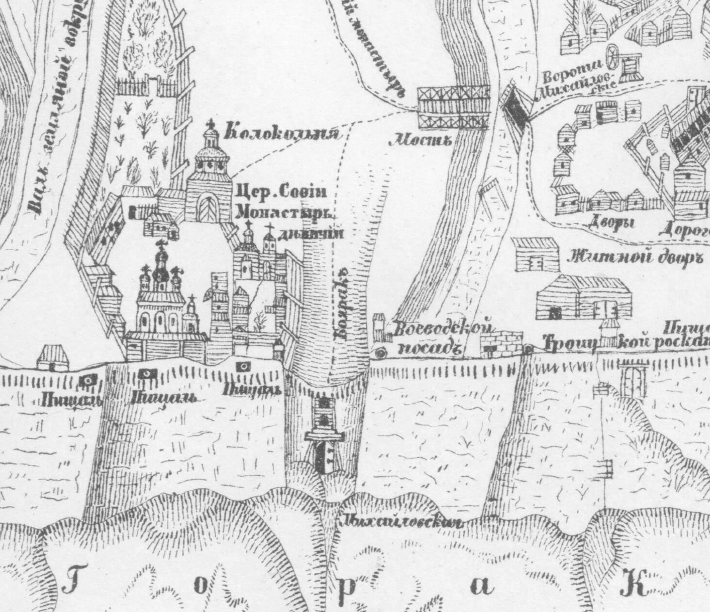
\includegraphics[width=\linewidth]{chast-colebanie-osnov/uvoz-borichev/1695-borichev.png}
\end{center}

Боярак проходил вдоль северо-западной (на плане – правой) стороны Михайловского монастыря и тянулся вглубь нынешней Михайловской площади, между МИДом и монастырской стеной. Уточнение – во время составления плана, к буераку выходил не Михайловский, но соседний Софиевский монастырь (не путать с Софией, она юго-западнее), переведенный затем на Кирилловские высоты под именем Богословского, где ныне Богуславский спуск.

Что значит наличие боярака на плане? Если овраг, то бишь дорога «Боричев», входит в верхнюю часть склона не просто так, а в буерак, являющийся продолжением оврага, то у нас получается более пологий угол наклона внутри оврага. Говоря с привязкой к современности, овраг от нижней Почтовой площади к верхней Михайловской был длиннее склона, как бы прорезал его и устремлялся вперед в Михайловскую, оставив позади край холма. Овраг с дорогой залегал глубже теперешнего. Потом его засыпали, о чем и сетовал Вигель. А боярак – это незасыпанный остаток оврага, с прежним уровнем дна.

Таким образом склон горы был круче, нежели дно оврага, который – как ясно из карты – вдавался глубоко в склон относительно его края. Чем больше угол наклона, тем короче дорога. Боярак удлинял дорогу и сбавлял угол наклона. Даже в засыпанном наверху бояраке в 18 веке была «Михайловская калитка» к нижележащему Михайловскому спуску, что сходил примерно к церкви Рождества, а значит лежал там же, где и Боричев.

Боричев овраг заканчивался примерно на пересечении Трехсвятительской улицы с площадью. Длина дороги по Боричеву была почти в два раза длиннее, нежели теперь. Значит, «увоз Боричев» был почти в два раза менее крутым, чем ныне.

Эта удивительная дорога в ущелье, природная или рукотворная, делала возможным подъем по ней относительно легким делом. Потому что иначе, 20 градусов подъема нынешнего склона там где фуникулер – это и пешком осилить тяжело, не говоря уже о ручной переноске грузов.

Любопытно, что Софиевский монастырь был перенесен в место, где поныне сохранилась, за Иорданским переулком, старинная дорога на Лукьяновку, которая в точности повторяет прежний Боричев, плавно вписываясь внутрь холма по желобу длинного оврага.

«Боярак» в верховьях Боричева просматривается на картах, после плана Ушакова, довольно долго. От крепостной стены у северо-западного берега оврага, к противоположному берегу с Михайловским монастырем (на уровне его юго-западного края) через овраг был перекинут мост, заметный еще на плане 1812 года. Спустя несколько десятилетий там уже ровное место.

По старинным фотографиям хорошо видно, как только за последние десятилетия 19 века и начало 20-го менялся склон, как в одних местах его крутизна сглаживалась террасами, а в других – напротив, с течением времени и земляных работ, увеличивалась. Представьте, сколь исказился рельеф с летописных времен! Петру I нужна наверху крепость? Склоны делаются обывистей, удобные подходы уничтожаются, овраги засыпаются, гора становится частью крепости, а склон естественным продолжением валов по его краю. Попробуй заберись! 

Затем эпоха строгости чуть смягчается, фортификационные сооружения в центре города мешают. Валы сравниваются, крепостные стены исчезают. Появляется необходимость в соединении Подола около Почтовой площади с верхним городом. Человек снова трудится, облегчает себе дорогу.

Вот пример. Два снимка, вид на фуникулер – или, как тогда говорили, Михайловский подъем – с Владимирской горки. 

На первом склон под церковью Василия, непосредственно справа от верхней площадки фуникулера, обрывист и дик. У опор под рельсами видны строительные леса либо дополнительные подпорки. Вдоль тропы слева – косой забор.

\begin{center}
\includegraphics[width=\linewidth]{chast-colebanie-osnov/uvoz-borichev/\myimgprefix fun-13.jpg}
\end{center}

И далее снимок, сделанный позже. Заметно, что участок под церковью сделан более пологим за счет уступов. За ним, в сторону Андреевской церкви, угол наклона тоже уменьшен – насыпали землю, она не заросла еще травой. Дальше снова дорожки по террасам на месте некогда сплошного склона. Слева же дорожка проходит иначе, и снабжена оградкой, а за нею ровненьким забором.

\begin{center}
\includegraphics[width=\linewidth]{chast-colebanie-osnov/uvoz-borichev/\myimgprefix mihpod04.jpg}
\end{center}
